% !TEX root = ../Documentation.tex

\section{Analysis}
\label{sec:analysis}

\subsection{System overview (MR)}
The requirements of the new parser have been described in the project planning \citenac{plan}.
Basically, both the old and the new parser must be able to make a conversion from a text file (ADL-script) to a parse tree (the P-structure).
\autoref{fig:data-flow-1} depicts this data flow.
%
\begin{figure}[htb!]
	\centering
	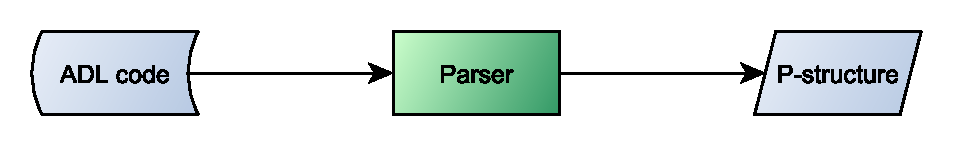
\includegraphics[width=0.586\textwidth]{Figures/DataFlow1}
	\caption{Relevant data flow for the Ampersand parsing component}
	\label{fig:data-flow-1}
\end{figure}

Often, the parsing component is separated into a lexer (that converts text to tokens) and the actual parser (that converts the tokens into the parse tree).
Since this separation is considered beneficial for both maintainability and performance \citeac{parsec}, we assumed from the beginning that the new Ampersand parser would be separated in this way.
This is depicted in \autoref{fig:data-flow-2}.
%
\begin{figure}[htb!]
	\centering
	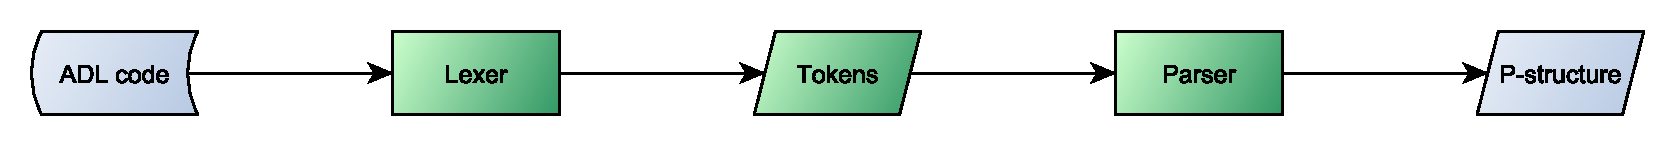
\includegraphics[width=1\textwidth]{Figures/DataFlow2}
	\caption{Data flow for the Ampersand lexing and parsing components}
	\label{fig:data-flow-2}
\end{figure}

In order to take the next steps and understand how the parser can be designed, we first take a look at the grammar in \autoref{subsec:analysis-grammar}, the parse tree in \autoref{subsec:analysis-parse-tree} and the parsing library in \autoref{subsec:analysis-parsing-lib}.
Afterwards, we analyze the lexer with the original token structure, so that we can define a new token structure, in \autoref{subsec:analysis-lexer}.
Finally, we analyze the parser in \autoref{subsec:analysis-parser} and the generated errors in \autoref{subsec:analysis-errors}.

\subsection{Grammar (M)}
\label{subsec:analysis-grammar}
\dict{EBNF}{Extended Backus-Naur Form}%
\dict{Extended Backus-Naur Form}{Notation technique for documenting context-free grammars}%
TODO: Show/describe the EBNF (maybe actual EBNF as attachment)

\subsection{Parse tree (D)}
\label{subsec:analysis-parse-tree}
TODO: Give a short description of the parse tree, and how it's different than the actual grammar.

\subsection{Parsing library (D)}
\label{subsec:analysis-parsing-lib}
TODO: reference the phase 3a decision to use parsec.

\subsection{Lexer (M)}
\label{subsec:analysis-lexer}
TODO: describe the possible improvements in the old lexer.

\subsubsection{Token structure}
TODO: Describe the old token strucure

\subsubsection{New token structure}
TODO: Develop a better token structure

\subsection{Parser (D)}
\label{subsec:analysis-parser}
TODO: describe the most important flaws in the old parser

\subsection{Errors (M)}
\label{subsec:analysis-errors}
TODO: show how the parser did not provide good errors, and how we could improve them.
